In this chapter, we study polynomial-time sampling algorithms. As
a primary motivation for much of the analysis, we consider the \emph{ball
walk}. 

\subsection*{The Ball Walk}

The simplest continuous algorithm for exploring space is Brownian
motion with the SDE $dx_{t}=dW_{t}$. To turn this into a sampling
algorithm, for a convex function $f$, we saw an extension using the
gradient of $f$, namely 
\[
dx_{t}=-\nabla f(x_{t})dt+\sqrt{2}dW_{t}
\]
which can be used to sample according to the density proportional
to $e^{-f}$. In this chapter we will begin with an even simpler method,
which does not need access to the gradient or assume differentiability,
only an oracle that can evaluate a function proportional to $Q$.

\begin{algorithm2e}[H]

\caption{$\mathtt{BallWalk}$}

\SetAlgoLined

Input: Step-size $\delta$, number of steps $T$, starting point $x_{0}$
in the support of target density $Q$.

Repeat $T$ times: at a point $x$,
\begin{enumerate}
\item Pick a random point $y$ in the $\delta$-ball centered at $x$.
\item Go to $y$ with probability $\min\left\{ 1,\frac{Q(y)}{Q(x)}\right\} $.
\item Otherwise, stay at $x$.
\end{enumerate}
\Return $x$.

\end{algorithm2e}
\begin{lem}
\emph{\label{lem:ballwalk-stationary}The distribution with density
$Q$ is stationary for the ball walk in a connected, compact full-dimensional
set, i.e., if the distribution of the current point $x$ has density
$Q$, it remains $Q$.}
\end{lem}

Under mild conditions, the distribution of the current point approaches
the target density $Q$. The main question is the rate of convergence,
which would allow us to bound the number of steps. Note that each
step involves only a function evaluation, to an oracle that outputs
the value of a function proportional to the desired density. To bound
the rate of convergence (and as a result the uniqueness of the stationary
distribution), we first develop some general tools.

\section{Basics of Markov chains}

For more detailed reading, including additional properties, see Section
1 of \cite{lovasz1993random}.

A Markov chain is defined using a $\sigma$-algebra $(K,{\cal A})$,
where $K$ is the state space and ${\cal A}$ is a set of subsets
of $K$ that is closed under complements and countable unions. For
each element $u$ of $K$, we have a probability measure $P_{u}$
on $(K,{\cal A})$, i.e., each set $A\in{\cal A}$ has a probability
$P_{u}(A)$. Informally, $P_{u}$ is the distribution obtained upon
taking one step from $u$. The triple $(K,{\cal A},\{P_{u}:u\in K\})$
along with a starting distribution $Q_{0}$ defines a Markov chain,
i.e., a sequence of elements of $K$, $w_{0},w_{1},\ldots$, where
$w_{0}$ is chosen from $Q_{0}$ and each subsequent $w_{i}$ is chosen
from $P_{w_{i-1}}$. The choice of $w_{i+1}$ depends only on $w_{i}$
and is independent of $w_{0},\ldots,w_{i-1}$. 
\begin{defn}
A distribution $Q$ on $(K,{\cal A})$ is called \emph{stationary}
if taking one step from it maintains the distribution, i.e., for any
$A\in{\cal A}$, 
\[
\int_{K}P_{u}(A)\,dQ(u)=Q(A).
\]
\end{defn}

\begin{defn}
A distribution $Q$ is \emph{atom-free} if there is no $x\in K$ with
$Q(x)>0$. 
\end{defn}

\begin{defn}
We say a Markov chain is \emph{time-reversible }if all of its stationary
distributions $Q$ satisfy \emph{detailed balance}:
\[
Q(u)P_{u}(v)=Q(v)P_{v}(u)\quad\forall u,v\in K
\]
where $Q(u)$ denotes the probability (density) of $Q$ at $u$ and
$P_{u}(v)$ denotes the probability (density) of transitioning from
$u$ to $v$.
\end{defn}

\begin{xca}
Show that if a distribution $Q$ satisfies detailed balance, then
it is stationary.
\end{xca}

\begin{xca}
Show Lemma \ref{lem:ballwalk-stationary}
\end{xca}

\begin{example*}
For the ball walk in a convex body, the state space $K$ is the convex
body, and $A$ is the set of all measurable subsets of $K$. The next
step distribution is 
\[
P_{u}(\{u\})=1-\frac{\vol\left(K\cap(u+\delta B_{n})\right)}{\vol(\delta B_{n})}
\]
and for any measurable subset $A$, 
\[
P_{u}(A)=\frac{\vol\left(A\cap(u+\delta B_{n})\right)}{\vol(\delta B_{n})}+1_{u\in A}(u)P_{u}(\{u\})
\]
The uniform distribution is stationary, i.e., $Q(A)=\frac{\vol(A)}{\vol(K)}$.
\end{example*}
\begin{defn}
The \emph{ergodic flow} of a subset $A$ with respect to the distribution
$Q$ is defined as 
\[
\Phi(A)=\int_{A}P_{u}(K\setminus A)\,dQ(u).
\]
A distribution $Q$ is stationary if and only if $\Phi(A)=\Phi(K\setminus A)$.
The existence and uniqueness of the stationary distribution $Q$ for
general Markov chains is a subject on its own. One way to ensure uniqueness
of a stationary distribution is to use \emph{lazy} Markov chains.
In a lazy version of a given Markov chain, at each step, with probability
$1/2$, we do nothing; with the remaining probability we take a step
according to the Markov chain. The next theorem is folklore.
\end{defn}

\begin{xca}
If $Q$ is stationary with respect to a lazy, ergodic Markov chain,
then it is the unique stationary distribution for that Markov chain.
\end{xca}

Informally, the mixing rate of a random walk is the number of steps
required to reduce some measure of the distance of the current distribution
to the stationary distribution by a constant factor. The following
notions will be useful for comparing two distributions $P,Q$.
\begin{enumerate}
\item Total variation distance is $d_{tv}(P,Q)=\sup_{A\in\mathcal{A}}|P(A)-Q(A)|.$
\item $L_{2}$ or $\chi^{2}$-distance of $P$ with respect to $Q$ is 
\[
\chi^{2}(P,Q)=\int_{K}\left(\frac{dP(u)}{dQ(u)}-1\right)^{2}dQ(u)=\int_{K}\left(\frac{dP(u)}{dQ(u)}\right)^{2}\,dQ(u)-1=\int_{K}\frac{dP(u)}{dQ(u)}\,dP(u)-1.
\]
\item KL-divergence: 
\[
d_{KL}(P,Q)=\int_{K}\log\frac{dP(u)}{dQ(u)}\,dP(u).
\]
\item Warmth: $P$ is said to be\emph{ $M$-warm} with respect to $Q$ if
$M=\sup_{A\in\mathcal{A}}\frac{P(A)}{Q(A)}.$
\end{enumerate}
\begin{defn}
We say that a distribution $P$ is \emph{absolutely continuous }with
respect to another distribution $Q$ if for any set $A$ for which
$Q(A)=0$ we also have $P(A)=0$. 
\end{defn}

The following relationships hold when $P$ is absolutely continuous
with respect to $Q$.
\begin{fact}
We have 
\[
2d_{TV}(P,Q)^{2}\le d_{KL}(P,Q)\le\chi^{2}(P,Q).
\]
\end{fact}


\subsection*{Convergence via Conductance}

Now we introduce an important tool to bound the rate of convergence
of $Q_{t}$, the distribution after $t$ steps to $Q$. Assume that
$Q$ is the unique stationary distribution. The \emph{conductance}
of a subset $A$ is defined as 
\[
\phi(A)=\frac{\Phi(A)}{\min\{Q(A),Q(K\setminus A)\}}
\]
and the conductance of the Markov chain is 
\[
\phi=\min_{A}\phi(A)=\min_{0<Q(A)\leq\frac{1}{2}}\frac{\int_{A}P_{u}(K\setminus A)\,dQ(u)}{Q(A)}.
\]
The \emph{local} conductance of an element $u$ is $\ell(u)=1-P_{u}(\{u\})$.

For any $0\leq s<\frac{1}{2}$, the $s$-conductance of a Markov chain
is defined as 
\[
\phi_{s}=\min_{A:s<Q(A)\leq\frac{1}{2}}\frac{\phi(A)}{Q(A)-s}.
\]

Ideally we would like to show that $d(Q_{t},Q)$, the distance between
the distribution after $t$ steps and the target $Q$ is monotonically
(and rapidly) decreasing. We consider 
\[
\sup_{A:Q(A)=x}Q_{t}(A)-Q(A)
\]
for each $x\in[0,1]$. To prove inductively that this quantity decreases,
let ${\cal G}_{x}$ be the set of functions defined as 
\[
{\cal G}_{x}=\left\{ g:K\rightarrow[0,1]\ :\ \int_{u\in K}g(u)\ dQ(u)=x\right\} .
\]
Using this, define 
\[
h_{t}(x)=\sup_{g\in{\cal G}_{x}}\int_{u\in K}g(u)\ (dQ_{t}(u)-dQ(u))=\sup_{g\in{\cal G}_{x}}\int_{u\in K}g(u)\ dQ_{t}(u)-x.
\]
This function is concave.
\begin{xca}
Show that the function $h_{t}$ is concave, and if $Q$ is atom-free
, then $h_{t}(x)=\sup_{A:Q(A)=x}Q_{t}(A)-Q(A)$ and the supremum
is achieved by some subset.

\begin{figure}[H]
\centering{}\includegraphics[width=0.7\textwidth]{Figures/Exercise_10\lyxdot 3}
\end{figure}
\end{xca}

If the target density $Q$ has atoms, i.e., points of positive probability,
then the function $g$ achieving $h$ might have a fractional value
at one atom.
\begin{lem}
Let $Q$ be atom-free and $t\geq1$. For any $0\leq x\leq1$, let
$y=\min\{x,1-x\}$. Then, 
\[
h_{t}(x)\le\frac{1}{2}h_{t-1}(x-2\phi y)+\frac{1}{2}h_{t-1}(x+2\phi y).
\]
\end{lem}

\begin{proof}
Assume that $0\leq x\leq\frac{1}{2}$. We construct two functions,
$g_{1}$ and $g_{2}$, and use these to bound $h_{t}(x)$. Let $A$
be a subset that achieves $h_{t}(x)$. Define

\[
g_{1}(u)=\begin{cases}
2P_{u}(A)-1 & \text{if }u\in A,\\
0 & \text{if }u\notin A,
\end{cases}\quad\text{ and }\quad g_{2}(u)=\begin{cases}
1 & \text{if }u\in A,\\
2P_{u}(A) & \text{if }u\notin A.
\end{cases}
\]
Note that $\frac{1}{2}(g_{1}+g_{2})(u)=P_{u}(A)$ for all $u\in K$,
which means that 
\[
\frac{1}{2}\int_{u\in K}g_{1}(u)\ dQ_{t-1}(u)+\frac{1}{2}\int_{u\in K}g_{2}(u)\,dQ_{t-1}(u)=\int_{u\in K}P_{u}(A)\,dQ_{t-1}(u)=Q_{t}(A).
\]
Since the walk is lazy, $P_{u}(A)\geq\frac{1}{2}$ if and only if
$u\in A$. Hence, the range of the functions $g_{1},g_{2}$ is $[0,1]$.
We let 
\[
x_{1}=\int_{u\in K}g_{1}(u)\ dQ(u)\quad\text{ and }\quad x_{2}=\int_{u\in K}g_{2}(u)\ dQ(u),
\]
then $g_{1}\in{\cal G}_{x_{1}}$ and $g_{2}\in{\cal G}_{x_{2}}$.
Moreover, 
\[
\frac{1}{2}(x_{1}+x_{2})=\frac{1}{2}\int_{u\in K}g_{1}(u)\ dQ(u)+\frac{1}{2}\int_{u\in K}g_{2}(u)\ dQ(u)=\int_{u\in K}P_{u}(A)\ dQ(u)=Q(A)=x.
\]
since $Q$ is stationary.
\begin{eqnarray*}
h_{t}(x) & = & Q_{t}(A)-Q(A)\\
 & = & \frac{1}{2}\int_{u\in K}g_{1}(u)\ dQ_{t-1}(u)+\frac{1}{2}\int_{u\in K}g_{2}(u)\ dQ_{t-1}(u)-Q(A)\\
 & = & \frac{1}{2}\int_{u\in K}g_{1}(u)\ (dQ_{t-1}(u)-dQ(u))+\frac{1}{2}\int_{u\in K}g_{2}(u)\ (dQ_{t-1}(u)-dQ(u))\\
 & \le & \frac{1}{2}h_{t-1}(x_{1})+\frac{1}{2}h_{t-1}(x_{2}).
\end{eqnarray*}

Next, 
\begin{eqnarray*}
x_{1} & = & \int_{u\in K}g_{1}(u)\ dQ(u)\\
 & = & 2\int_{u\in A}P_{u}(A)\ dQ(u)-\int_{u\in A}dQ(u)\\
 & = & 2\int_{u\in A}(1-P_{u}(K\setminus A))\ dQ(u)-x\\
 & = & x-2\int_{u\in A}P_{u}(K\setminus A)\ dQ(u)\\
 & = & x-2\Phi(A)\\
 & \le & x-2\phi x\\
 & = & x(1-2\phi).
\end{eqnarray*}
Thus we have, $x_{1}\leq x(1-2\phi)\leq x\leq x(1+2\phi)\leq x_{2}.$
Since $h_{t-1}$ is concave, the chord from $x_{1}$ to $x_{2}$ on
$h_{t-1}$ lies below the chord from $[x(1-2\phi),x(1+2\phi)${]}.
Therefore, 
\[
h_{t}(x)\le\frac{1}{2}h_{t-1}(x(1-2\phi))+\frac{1}{2}h_{t-1}(x(1+2\phi)).
\]
\end{proof}
A proof along the same lines implies the following generalization.
\begin{lem}
Let $Q$ be atom-free and $0\leq s\leq1$. For any $s\leq x\leq1-s$,
let $y=\min\{x-s,1-x-s\}$. Then for any integer $t>0$, 
\[
h_{t}(x)\leq\frac{1}{2}h_{t-1}(x-2\phi_{s}y)+\frac{1}{2}h_{t-1}(x+2\phi_{s}y).
\]
\end{lem}

These results can be extended to the case when $Q$ has atoms with
slightly weaker bounds \cite{lovasz1993random}.
\begin{thm}
\label{thm:s-mixing}Let $0\leq s\leq1$ and $C_{0}$ and $C_{1}$
be such that 
\[
h_{0}(x)\le C_{0}+C_{1}\min\{\sqrt{x-s},\sqrt{1-x-s}\}.
\]
 Then 
\[
h_{t}(x)\le C_{0}+C_{1}\min\{\sqrt{x-s},\sqrt{1-x-s}\}\left(1-\frac{\phi^{2}_{s}}{2}\right)^{t}.
\]
\end{thm}

\begin{proof}
Assume that $x-s\in[0,1/2]$. The proof is by induction on $t$. The
base case is by assumption. For the general case, we write

\begin{align*}
h_{t}(x) & \leq\frac{1}{2}h_{t-1}(x-2\phi_{s}(x-s))+\frac{1}{2}h_{t-1}(x+2\phi_{s}(x-s))\\
 & \le\frac{1}{2}C_{0}+\frac{1}{2}C_{1}\sqrt{(x-s)(1-2\phi_{s})}\left(1-\frac{\phi^{2}_{s}}{2}\right)^{t-1}+\frac{1}{2}C_{0}+\frac{1}{2}C_{1}\sqrt{(x-s)(1+2\phi_{s})}\left(1-\frac{\phi^{2}_{s}}{2}\right)^{t-1}\\
 & \le C_{0}+C_{1}\left(\frac{1}{2}\sqrt{(x-s)(1-2\phi_{s})}+\frac{1}{2}\sqrt{(x-s)(1+2\phi_{s})}\right)\left(1-\frac{\phi^{2}_{s}}{2}\right)^{t-1}\\
 & \le C_{0}+C_{1}\sqrt{x-s}\left(1-\frac{\phi^{2}_{s}}{2}\right)^{t}.
\end{align*}
\end{proof}
This leads to the following useful corollaries.
\begin{cor}
\label{cor:s-mixing}We have
\begin{enumerate}
\item Let $M=\sup_{A}Q_{0}(A)/Q(A)$. Then, 
\[
d_{TV}(Q_{t},Q)\le\sqrt{M}\left(1-\frac{\phi^{2}}{2}\right)^{t}.
\]
\item Let $0<s\leq\frac{1}{2}$ and $H_{s}=\sup\{|Q_{0}(A)-Q(A)|:Q(A)\leq s\}$.
Then, 
\[
d_{TV}(Q_{t},Q)\leq H_{s}+\frac{H_{s}}{s}\left(1-\frac{\phi^{2}_{s}}{2}\right)^{t}.
\]
\item Let $M=\chi^{2}(Q_{0},Q)$. Then for any $\varepsilon>0$, 
\[
d_{TV}(Q_{t},Q)\leq\varepsilon+\sqrt{\frac{M}{\varepsilon}}\left(1-\frac{\phi^{2}}{2}\right)^{t}.
\]
\end{enumerate}
\end{cor}

The next theorem will allow us to provide a more uniform \emph{contraction
}bound for the $\chi^{2}$-divergence of the $t$-step distribution.
The Markov transition operator $M$ for a Markov scheme given by state
space $\Omega$ and next-step distributions $\left\{ P_{u}(.)\right\} $
is a map from square-integrable functions to square-integrable functions
over $\Omega$, defined as follows
\[
Mf(u)=\int_{\Omega}f(v)\,dP_{u}(v)
\]
the expected value of $f(w_{i+1})$ under the Markov chain given that
$w_{i}=u$. 
\begin{thm}
\label{thm:transition-operator-norm}For a lazy, time-reversible Markov
chain with transition operator $M$, stationary distribution $Q$
and conductance $\phi$, and any $f:\Omega\rightarrow\R$ that is
square-integrable with $\E_{Q}(f)=0$, we have 
\[
\left\langle f,Mf\right\rangle =\int_{\Omega}f(x)Mf(x)\,dQ(x)\le\left(1-\frac{\phi^{2}}{4}\right)\int_{\Omega}f(x)^{2}\,dQ(x)=\left(1-\frac{\phi^{2}}{4}\right)\norm f^{2}.
\]
\end{thm}

\begin{proof}
The core of this proof is Cheeger's classical inequality. Let $r$
be such that $Q(\{x:f(x)>r\})\le1/2$ and $Q(\{x:f(x)<r\})\le1/2$.
Let $g(x)=\max\{f(x)-r,0\}$. We then have
\[
\int_{\Omega}g(x)^{2}\,dQ(x)\ge\frac{1}{2}\int_{\Omega}(f(x)-r)^{2}\,dQ(x)=\frac{1}{2}\norm f^{2}+\frac{1}{2}r^{2}\ge\frac{1}{2}\norm f^{2}
\]
where if needed we replace $f$ with $-f$. 

Next, defining $A(t)=\{x:g(x)^{2}\ge t\}$, and using $\E_{Q}(h(x))=\int^{\infty}_{t=0}\Pr_{Q}(h(x)\ge t)\,dt$
for any nonnegative function $h$, we have 
\begin{align*}
\int_{\Omega}\int_{\Omega}\left|g(x)^{2}-g(y)^{2}\right|\,dP_{y}(x)\,dQ(y) & =2\int_{\Omega}\int_{A(g(y)^{2})}\left(g(x)^{2}-g(y)^{2}\right)\,dP_{y}(x)\,dQ(y)\\
 & =2\int_{\Omega}\int^{\infty}_{g(y)^{2}}P_{y}(A(t))\,dt\,dQ(y)\\
 & =2\int^{\infty}_{0}\int_{\Omega\setminus A(t)}P_{y}(A(t))\,dQ(y)\,dt\\
 & \ge2\phi\int^{\infty}_{0}Q(A(t))\,dt\\
 & =2\phi\int_{\Omega}g(x)^{2}\,dQ(x)\\
 & =2\phi\norm g^{2}
\end{align*}
noting that for $t\ge0$, we have $Q(A(t))\le1/2$ by the choice of
$r$. 

By Cauchy-Schwarz, we also have
\begin{align*}
\left(\int_{\Omega}\int_{\Omega}\left|g(x)^{2}-g(y)^{2}\right|\,dP_{y}(x)\,dQ(y)\right)^{2} & \le\int_{\Omega}\int_{\Omega}\left(g(x)-g(y)\right)^{2}\,dP_{y}(x)\,dQ(y)\int_{\Omega}\int_{\Omega}\left(g(x)+g(y)\right)^{2}\,dP_{y}(x)\,dQ(y).
\end{align*}
We can bound the second term as
\begin{align*}
\int_{\Omega}\int_{\Omega}\left(g(x)+g(y)\right)^{2}\,dP_{y}(x)\,dQ(y) & \le2\int_{\Omega}\int_{\Omega}\left(g(x)^{2}+g(y)^{2}\right)\,dP_{y}(x)\,dQ(y)\\
 & =4\int_{\Omega}g(x)^{2}\,dQ(x)\\
 & =4\norm g^{2}.
\end{align*}
Putting these together, 
\begin{align*}
\int_{\Omega}\int_{\Omega}\left(g(x)-g(y)\right)^{2}\,dP_{y}(x)\,dQ(y) & \ge\frac{4\phi^{2}\norm g^{4}}{4\norm g^{2}}\ge\phi^{2}\norm g^{2}\ge\frac{\phi^{2}}{2}\norm f^{2}.
\end{align*}
Hence, 
\[
\norm f^{2}-\langle f,Mf\rangle=\frac{1}{2}\int_{\Omega}\int_{\Omega}\left(f(x)-f(y)\right)^{2}\,dP_{y}(x)\,dQ(y)\ge\frac{\phi^{2}}{4}\norm f^{2}
\]
which proves the conclusion.
\end{proof}
This has an immediate corollary.
\begin{cor}
For a lazy, time-reversible Markov chain with stationary distribution
$Q$ and conductance $\phi$, we have 
\[
\chi^{2}(Q_{t},Q)\le\left(1-\frac{\phi^{2}}{4}\right)^{2t}\chi^{2}(Q_{0},Q).
\]
\end{cor}

\begin{proof}
Theorem \ref{thm:transition-operator-norm} implies that the transition
operator $M$ satisfies 
\[
\norm M\le1-\frac{\phi^{2}}{4}.
\]
As a result, we have 
\[
\langle Mf,Mf\rangle\le\left(1-\frac{\phi^{2}}{4}\right)^{2}\langle f,f\rangle.
\]
By setting $f(x)=\frac{dQ_{t-1}(x)}{dQ(x)}-1$, we get 
\[
\chi^{2}\left(Q_{t},Q\right)\le\left(1-\frac{\phi^{2}}{4}\right)^{2}\chi^{2}(Q_{t-1},Q).
\]
 
\end{proof}


\subsection*{Convergence via Log-Sobolev}

For a warm start, the convergence rate established by conductance
is asymptotically optimal in many cases of interest, including the
ball walk for a convex body. However, when the starting distribution
is more focused, e.g., a single point, then there is a significant
starting penalty, usually a factor of the dimension or larger. One
way to avoid this is to observe that the conductance of smaller subsets
is in fact even higher and that one does not need to pay this large
starting penalty. A classical technique in this regard is the log-Sobolev
constant. For a Markov chain with stationary density $Q$ and transition
operator $P$, we can define it as follows. 
\[
\rho=\inf_{g:\mbox{\mbox{smooth}, \ensuremath{\int g(x)^{2}dQ(x)=1}}}\frac{\int_{x,y\in K}\left(g(x)-g(y)\right)^{2}P(x,y)dQ(x)}{\int g(x)^{2}\log g(x)^{2}dQ(x)}.
\]

This parameter allows us to show convergence of the current distribution
to the target in relative entropy. Recall that the relative entropy
of a distribution $P$ with respect to a distribution $Q$ is 
\[
H_{Q}(P)=\int_{K}P(x)\log\frac{P(x)}{Q(x)}dQ(x).
\]

\begin{thm}
For a Markov chain with distribution $Q_{t}$ at time $t$, and log-Sobolev
parameter $\rho$, we have 
\[
H_{Q}(Q_{t})\le e^{-2\rho t}H_{Q}(Q_{0}).
\]

\end{thm}


\section{Conductance of the Ball Walk}

In this section we bound the conductance of the ball walk when applied
to the indicator function of a convex body. At first glance, the ball
walk is not an efficient algorithm, even for uniformly sampling a
convex body. The reason is simply that the local conductance could
be exponentially small (consider a point close to the vertex of a
polyhedron). We can get around this in two ways. The first, which
is simpler, but less efficient is to ``smooth'' the convex body
by taking the Minkowski sum with a small Euclidean ball, i.e., replace
$K$ with $K+\alpha B^{n}$.

\begin{figure}[H]
\begin{centering}
\includegraphics[width=0.75\columnwidth]{Figures/Exercise_10\lyxdot 9}
\par\end{centering}
\end{figure}

\begin{xca}
Let $K$ be a convex body in $\R^{n}$ containing the unit ball. Show
that (a) $\vol(K+\alpha B^{n})\leq(1+\alpha)^{n}\vol(K)$ and (b)
with $\delta=\alpha/\sqrt{n}$ the local conductance of every point
in $K+\alpha B^{n}$ is at least an absolute constant.
\end{xca}

Using the exercise, it suffices to set $\alpha=1/n$, so that a sample
from $K+\alpha B^{n}$ has a large probability of being in $K$ and
then $\delta=1/n^{3/2}$.

The second approach is to show that the local conductance is in fact
large almost everywhere, and if the starting distribution is ``warm''
then these points can effectively be ignored. This will allow us to
make $\delta$ much larger, namely $\delta=1/\sqrt{n}.$ Larger step
sizes should allow us to prove faster mixing.

To convey the main ideas of the analysis, we focus on the first approach
here. The goal is to show that the conductance of any subset is large,
i.e., the probability of crossing over in one step is at least proportional
to the measure of the set or its complement, whichever is smaller.
First, we argue that the one-step distributions of two points will
have a significant overlap if the points are sufficiently close.
\begin{lem}[One-step overlap]
\label{lem:ONESTEP} Let $u,v\in K$ such that $\ell(u),\ell(v)\ge\ell$
and $\norm{u-v}\le\frac{t\delta}{\sqrt{n}}$. Then the one-step distributions
from them satisfy $d_{TV}(P_{u},P_{v})\le1+t-\ell$.

\begin{figure}[H]

\centering{}\includegraphics[width=0.5\columnwidth]{Figures/Thrm_10\lyxdot 12}\caption{\label{fig:fully-contained} One-step overlap fully contained in K}
\end{figure}
\end{lem}

\begin{proof}
First assume that $\ell=1$. This means that the balls of radius $\delta$
centered at $u$ and $v$ are fully contained in $K$. The TV distance
between these distributions is bounded by $\vol(u+\delta B^{n}\setminus v+\delta B^{n})=\vol(v+\delta B^{n}\setminus u+\delta B^{n})$
divided by $\vol(\delta B^{n})$. This is exactly the volume of a
band of thickness $\norm{u-v}$ centered at the center of $\delta B^{n}$
(see Fig.~\ref{fig:fully-contained}). This has relative volume at
most $t$, proving the lemma under the assumption that $\ell=1$.
For the general case, we note that when the balls are intersected
with a convex body, the increase in the TV distance is at most the
probability that there is no proper move at $u$ (or $v$), i.e.,
$1-\ell$. This completes the proof. 

\begin{figure}[H]

\begin{centering}
\includegraphics[width=0.5\columnwidth]{Figures/Thrm_10\lyxdot 12(1)}\caption{One-step overlap intersected by K}
\par\end{centering}
\end{figure}
\end{proof}
Setting $t=\ell/2$, this says that if the total variation distance
between the one-step distributions from $u,v$ is greater than $1-\ell/2$,
then the distance between them is at least $\frac{\ell\delta}{2\sqrt{n}}$.
What this effectively says is that points close to the internal boundary
of a subset are likely to cross over to the other side. To complete
a proof we would need to show that the internal boundary of any subset
is large if the subset (or its complement) is large, a purely geometric
property.
\begin{defn}
For two sets $A,B\subseteq\Rn$, let $d(A,B)=\inf_{x\in A,y\in B}||x-y||_{2}$.
The \emph{isoperimetric ratio }of a convex body $K$ is defined to
be 
\[
\inf_{(S_{1},S_{2},S_{3})\in P}\frac{\text{\ensuremath{\vol}}(S_{3})}{d(S_{1},S_{2})\min\left\{ \text{\ensuremath{\vol}}(S_{1}),\vol(S_{2})\right\} }
\]
where $P$ is the set of all partitions of $K$ into three measurable
sets, each of nonzero volume. We can generalize this definition for
a logconcave measure $\mu$ by replacing $\vol(S_{1}),\vol(S_{2}),\vol(S_{3})$
with $\mu(S_{1}),\mu(S_{2}),\mu(S_{3})$, respectively, and instead
letting $P$ be the set of partitions of the support of $\mu$ into
three sets.
\end{defn}

\begin{thm}[Isoperimetry]
\label{thm:isoD} The isoperimetric ratio of any convex body is at
least $\frac{2}{D}$. That is, let $S_{1},S_{2},S_{3}$ be a partition
of a convex body $K$ of diameter $D$. Then,
\[
\vol(S_{3})\ge\frac{2}{D}d(S_{1},S_{2})\min\left\{ \vol(S_{1}),\vol(S_{2})\right\} .
\]
\end{thm}

In fact, the isoperimetric ratio of any logconcave measure is also
$\frac{2}{D}$, where $D$ is the diameter of the measure's support.
We will discuss this and other extensions in detail later. But first
we bound the conductance.

\begin{figure}[H]
\centering{}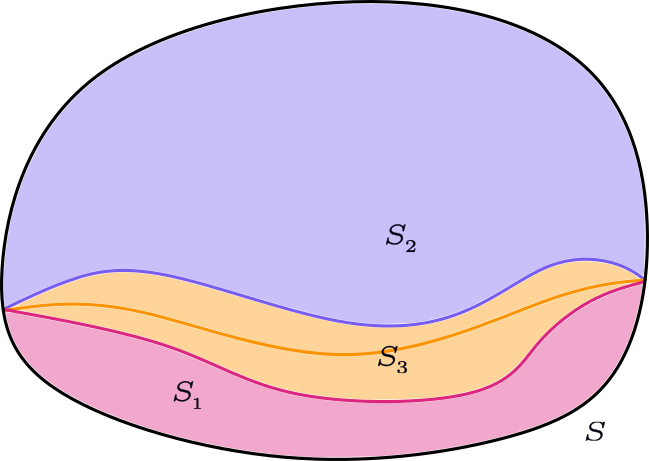
\includegraphics[width=0.55\columnwidth]{Figures/Partitions}\caption{Partitions of convex body}
\end{figure}

\begin{thm}
\label{thm:ball_walk_cond}Let $K$ be a convex body in $\R^{n}$
of diameter $D$ containing the unit ball and with every $u\in K$
having $\ell(u)\ge\ell.$ Then the conductance of the ball walk on
$K$ with step size $\delta$ is 
\[
\Omega\left(\frac{\ell^{2}\delta}{\sqrt{n}D}\right).
\]
\end{thm}

\begin{proof}
Let $K=S_{1}\cup S_{2}$ be a partition into measurable sets. We will
prove that

\begin{eqnarray}
\int_{S_{1}}P_{x}(S_{2})\,dx & \ge & \frac{\ell^{2}\delta}{16\sqrt{n}D}\min\{\vol(S_{1}),\vol(S_{2})\}\label{COND}
\end{eqnarray}
Note that since the uniform distribution is stationary, 
\[
\int_{S_{1}}P_{x}(S_{2})\,dx=\int_{S_{2}}P_{x}(S_{1})\,dx.
\]

Consider the points that are ``deep'' inside these sets, i.e., unlikely
to jump out of the set: 
\[
S_{1}'=\left\{ x\in S_{1}:P_{x}(S_{2})<\frac{\ell}{4}\right\} \mbox{ and }S_{2}'=\left\{ x\in S_{2}:P_{x}(S_{1})<\frac{\ell}{4}\right\} .
\]
Let $S_{3}'$ be the rest i.e., $S_{3}'=K\setminus S_{1}'\setminus S_{2}'$.

Suppose $\vol(S_{1}')<\vol(S_{1})/2$. Then 
\[
\int_{S_{1}}P_{x}(S_{2})\,dx\ge\frac{\ell}{4}\vol(S_{1}\setminus S_{1}')\geq\frac{\ell}{8}\vol(S_{1})
\]
which proves (\ref{COND}).

So we can assume that $\vol(S_{1}')\geq\vol(S_{1})/2$ and similarly
$\vol(S_{2}')\geq\vol(S_{2})/2$. Now, for any $u\in S_{1}'$ and
$v\in S_{2}'$, 
\[
||P_{u}-P_{v}||_{tv}\geq1-P_{u}(S_{2})-P_{v}(S_{1})>1-\frac{\ell}{2}.
\]
Applying Lemma \ref{lem:ONESTEP} with $t=\ell/2$, we get that 
\[
|u-v|\geq\frac{\ell\delta}{2\sqrt{n}}.
\]
Thus $d(S_{1}',S_{2}')\geq\ell\delta/(2\sqrt{n})$. Applying Theorem
\ref{thm:isoD} to the partition $S_{1}',S_{2}',S_{3}'$, we have
\begin{eqnarray*}
\vol(S_{3}') & \geq & \frac{\ell\delta}{\sqrt{n}D}\min\{\vol(S_{1}'),\vol(S_{2}')\}\\
 & \geq & \frac{\ell\delta}{2\sqrt{n}D}\min\{\vol(S_{1}),\vol(S_{2})\}.
\end{eqnarray*}
We can now prove (\ref{COND}) as follows: 
\begin{eqnarray*}
\int_{S_{1}}P_{x}(S_{2})\,dx & = & \frac{1}{2}\int_{S_{1}}P_{x}(S_{2})\,dx+\frac{1}{2}\int_{S_{2}}P_{x}(S_{1})\,dx\\
 & \ge & \frac{1}{2}\vol(S_{3}')\frac{\ell}{4}\\
 & \ge & \frac{\ell^{2}\delta}{16\sqrt{n}D}\min\{\vol(S_{1}),\vol(S_{2})\}.
\end{eqnarray*}

\begin{figure}[H]

\centering{}\includegraphics[width=0.75\columnwidth]{Figures/Lemma_10\lyxdot 10}
\end{figure}

\begin{figure}[H]

\begin{centering}
\includegraphics[width=0.3\columnwidth]{Figures/Lemma_10\lyxdot 10(1)}
\par\end{centering}
\end{figure}
\end{proof}
\begin{cor}
The ball walk in a convex body with local conductance at least $\ell$
everywhere has mixing rate $O(\frac{nD^{2}}{\delta^{2}\ell^{4}})$.
\end{cor}

Using the construction above of adding a small ball to every point
of $K$ gives a lower bound of $\delta=1/n^{3/2}$ and $\ell=\Omega(1)$
and thus a polynomial bound of $O(n^{4}D^{2})$ on the mixing time.
As we will see presently, this can be improved to $n^{2}D^{2}$ by
avoiding the blow-up, and analyzing the \emph{average }local conductance.
The example of starting near a corner (say of a hypercube) shows that
this cannot work in general; however, from a \emph{warm} start, it
will suffice to bound the average local conductance rather than the
minimum. 

\subsection*{Warm Start and $s$-Conductance}

In this section we give a better bound for the conductance of sufficiently
large subsets resulting in the following bound on the mixing rate
of the ball walk.
\begin{thm}
\label{thm:ballwalk_warmstart} From an $O(1)$-warm start, the ball
walk in a convex body with isoperimetric coefficient $\psi$ and containing
a unit ball has a mixing rate of $O(n^{2}/\psi^{2})$ steps. In particular,
if the convex body has diameter $D$, the mixing rate is $O(n^{2}D^{2})$. 
\end{thm}

This is based on two ideas: (1) most points of a convex body containing
a unit ball have large local conductance and we can use $\delta=1/\sqrt{n}$
instead of $1/n^{3/2}$, (2) the $s$-conductance is large and hence
the walk mixes from a suitably warm start.
\begin{lem}
\label{lem:avg-local-conductance} Let $K$ be a convex body containing
a unit ball. For the ball walk with $\delta$ step size, let $K_{\delta}=\left\{ u\in K:\:\ell(u)\ge\frac{3}{4}\right\} $.
Then $K_{\delta}$ is a convex set and $\vol(K_{\delta})\ge(1-2\delta\sqrt{n})\vol(K).$
\end{lem}

\begin{xca}
Prove the first part of the previous lemma.
\end{xca}

The proof of the above lemma will use the following bound on crossing
the boundary of $K$. 
\begin{lem}
Let $L$ be any measurable subset of the boundary of a convex body
$K$ and $S_{L}=\{(x,y):x\in K,y\not\in K,\norm{x-y}\le\delta,[x,y]\cap L\neq\emptyset\}$.
Then, we have 
\[
\vol_{2n}(S_{L})\le\frac{\delta}{(n+1)}\frac{\vol(B^{n-1})}{\vol(B^{n})}\vol_{n-1}(L)\vol(\delta B^{n}).
\]
\end{lem}

\begin{proof}
It suffices to consider the case when $L$ is infinitesimally small;
and then we can assume that the surface of $K$ is locally a hyperplane
and compute the measure of $S_{L}$ explicitly. 
\end{proof}
\begin{thm}
The $s$-conductance of the ball walk with $\delta=\frac{s}{4\sqrt{n}}$
step size in a convex body $K$ with isoperimetric coefficient $\psi$
and containing the unit ball satisfies 
\[
\phi_{s}\gtrsim\frac{s\psi}{n}.
\]
\end{thm}

This proof is similar to that of Theorem \ref{thm:ball_walk_cond},
with one important extension. Rather than applying the argument to
a partition of the original convex body $K$, we restrict the argument
to $K_{\delta}$, the set of points in $K$ that have high local conductance.
Since this subset takes up most of $K$, and is convex, we will be
able to use its isoperimetry to lower bound the conductance. 
\begin{proof}
As before, we consider the following partition of $K$. Let $K=S_{1}\cup S_{2}$
be a partition into measurable sets. We will prove that

\begin{eqnarray}
\int_{S_{1}}P_{x}(S_{2})\,dx & \ge & \frac{\delta\psi}{C\sqrt{n}}\min\{\vol(S_{1})-\frac{s}{2},\vol(S_{2})-\frac{s}{2}\}\label{COND-1}
\end{eqnarray}
Since the uniform distribution is stationary, 
\[
\int_{S_{1}}P_{x}(S_{2})\,dx=\int_{S_{2}}P_{x}(S_{1})\,dx.
\]

Consider the points that are ``deep'' inside these sets: 
\[
S_{1}'=\left\{ x\in S_{1}:P_{x}(S_{2})<\frac{1}{8}\right\} \mbox{ and }S_{2}'=\left\{ x\in S_{2}:P_{x}(S_{1})<\frac{1}{8}\right\} .
\]
Let $S_{3}'$ be the rest i.e., $S_{3}'=K\setminus S_{1}'\setminus S_{2}'$.
Recall that 
\[
K_{\delta}=\left\{ x\in K:\ell(x)\ge\frac{3}{4}\right\} 
\]
and define $S_{i}''=S_{i}'\cap K_{\delta}.$ Note that by Lemma \ref{lem:avg-local-conductance},
for $\delta\le s/(4\sqrt{n})$, 
\[
\vol(S_{i}'')\ge\vol(S_{i}')-s.
\]

Suppose $\vol(S_{1}'')<\vol(S_{1}\cap K_{\delta})/2$. Then 
\[
\int_{S_{1}}P_{x}(S_{2})\,dx\ge\frac{1}{8}\vol(S_{1}\cap K_{\delta}\setminus S_{1}'')\geq\frac{1}{16}\vol(S_{1}\cap K_{\delta})\ge\frac{1}{16}\left(\vol(S_{1})-\frac{s}{2}\right)
\]
which proves (\ref{COND-1}).

So we can assume that $\vol(S_{1}'')\geq\vol(S_{1}\cap K_{\delta})/2$
and similarly $\vol(S_{2}'')\geq\vol(S_{2}\cap K_{\delta})/2$. Now,
for any $u\in S_{1}''$ and $v\in S_{2}''$, 
\[
d_{TV}(P_{u},P_{v})\geq1-P_{u}(S_{2})-P_{v}(S_{1})>1-\frac{1}{4}.
\]
Applying Lemma \ref{lem:ONESTEP} with $t=3/8$, we get that 
\[
|u-v|\geq\frac{3\delta}{8\sqrt{n}}.
\]
Thus $d(S_{1}'',S_{2}'')\geq3\delta/(8\sqrt{n})$. Using the bound
on the isoperimetric coefficient applied to the partition $S_{1}'',S_{2}'',S_{3}''$
of $K_{\delta}$, we have 
\begin{eqnarray*}
\vol(S_{3}'') & \geq & \frac{3\delta\psi}{8\sqrt{n}}\min\{\vol(S_{1}''),\vol(S_{2}'')\}\\
 & \geq & \frac{3\delta\psi}{16\sqrt{n}}\min\{\vol(S_{1})-\frac{s}{2},\vol(S_{2})-\frac{s}{2}\}.
\end{eqnarray*}
We can now prove (\ref{COND-1}) as follows: 
\begin{eqnarray*}
\int_{S_{1}}P_{x}(S_{2})\,dx & = & \frac{1}{2}\int_{S_{1}}P_{x}(S_{2})\,dx+\frac{1}{2}\int_{S_{2}}P_{x}(S_{1})\,dx\\
 & \ge & \frac{1}{2}\vol(S_{3}'')\cdot\frac{1}{8}\\
 & \ge & \frac{3\delta\psi}{256\sqrt{n}}\min\{\vol(S_{1})-\frac{s}{2},\vol(S_{2})-\frac{s}{2}\}
\end{eqnarray*}
which implies that the conductance is at least $3s\psi/(1024n)$.
\end{proof}
The mixing rate then follows by applying Theorem \ref{thm:s-mixing}
and Corollary \ref{cor:s-mixing}.

\subsection*{Tightness of the bound}

The mixing rate of $O(n^{2}D^{2})$ for the ball walk is in fact the
best possible even from a warm start (with the assumption of a unit
ball inside the convex body and diameter $D$). To see this, consider
a cylinder whose cross-section is a unit ball and axis is $[0,D]$
along $e_{1}$. Suppose the starting distribution is uniform in the
part of the cylinder in $[0,D/3]$. Then we claim that to reach the
opposite third of the cylinder needs $\Omega(n^{2}D^{2})$ steps with
high probability. Each step has length at most $\delta$ in a random
direction, and this is about $\delta/\sqrt{n}$ along $e_{1}$. Viewing
this as an unbiased random walk along $e_{1}$, the effective diameter
is $D/(\delta/\sqrt{n})$ and hence the number of steps to cross an
interval of length $D/3$ is $\Omega(nD^{2}/\delta^{2})=\Omega(n^{2}D^{2})$.
\begin{xca}
Prove the above claim rigorously.
\end{xca}


\subsection*{Speedy walk}

In the above analysis of the ball walk, the dependence on the error
parameter $\varepsilon$, the distance to the target distribution,
is polynomial in $1/\varepsilon$ rather than its logarithm. The speedy
walk is a way to improve the analysis. In the speedy walk, at a point
$x$, we sample the next step uniformly from the intersection of $(x+\delta B^{n})\cap K$.
The resulting Markov chain is the subsequence of \emph{proper }steps
of the ball walk.
\begin{xca}
Show that the stationary density of the speedy walk in a convex body
is proportional to the local conductance.
\end{xca}

\begin{thm}
The conductance of the speedy walk is $\Omega(1/(nD))$.
\end{thm}

To analyze the ball walk, we then need to show that the number of
``wasted'' steps is not too many. This follows from the assumption
of a warm start and Lemma \ref{lem:avg-local-conductance}.

\section{Generating a warm start}

To get the mixing rate of $O(n^{2}D^{2})$, we need a warm start,
i.e., a distribution whose density at any point is within $O(1)$
of the target density.

\begin{algorithm2e}[H]

\caption{$\mathtt{Warm\,Start}$}

\SetAlgoLined

Input: membership oracle for $K$ such that $B^{n}\subseteq K\subseteq DB^{n}$.

Let $x$ be a random point in $B^{n}.$ Define $K_{i}=2^{i/n}B^{n}\cap K$.

\For{$i=1,\cdots,n\log D$}{
\begin{enumerate}
\item Use ball walk from $x$ to generate random point $y$ in $K_{i}$.
\item Set $x=y$.
\end{enumerate}
}

\Return $x$.

\end{algorithm2e}

Since $K_{i+1}\subseteq2^{1/n}K_{i}$, we have $\vol(K_{i+1})\le2\vol(K_{i})$
and hence a $2$-warm start is maintained. Once we have a random point
from $K$, subsequent random points can be generated by simply continuing
the ball walk; thus the cost of the warm start is only for the first
sample.

\section{Isotropic Transformation}

The complexity of sampling with the ball walk is polynomial in $n,D$
and $\log(1/\varepsilon)$ to get within $\varepsilon$ of the target
density. This is not a polynomial algorithm since the dependence is
on $D$ and not $\log D$. To get a polynomial algorithm, we need
one more ingredient.

We say that a distribution $Q$ is \emph{isotropic} if $\E_{Q}(x)=0$
and $\E_{Q}(xx^{T})=I$, i.e., the mean is zero and the covariance
matrix (exists and) is the identity. We say that the distribution
is $C$-isotropic if the eigenvalues of its covariance matrix are
in $[\frac{1}{C},C]$. An affine transformation is said to be an \emph{isotropic
transformation} if the resulting distribution is isotropic.

Any distribution with bounded second moments has an isotropic transformation.
It is clear that satisfying the first condition is merely a translation,
so assume the mean is zero. For the second, suppose the covariance
matrix is $\E_{Q}(xx^{T})=A$. Then consider $y=A^{-1/2}x$. It is
easy to see that 
\[
\E(yy^{T})=A^{-1/2}\E\left(xx^{T}\right)A^{-1/2}=I.
\]

For convex bodies, isotropic position comes with a strong guarantee.
\begin{thm}
\label{thm:isotropic-r-R}For a convex body in isotropic position
(i.e., the uniform distribution over the body is isotropic), we have
\[
\sqrt{\frac{n+2}{n}}B^{n}\subseteq K\subseteq\sqrt{n(n+2)}B^{n}.
\]
\end{thm}

\begin{xca}
Show Theorem \ref{thm:isotropic-r-R} up to absolute constants, i.e.,
show that for any convex body in isotropic position, it contains and
is contained in origin-centered balls of radii $\Omega(1)$ and $O(n)$,
respectively. Moreover, give an isotropic convex body where both of
these bounds are tight.
\end{xca}

Thus the effective diameter is $O(n)$. If we could place a convex
body in isotropic position before sampling, we would have a poly($n$)
algorithm. In fact, it is even better than this as most points are
within distance $O(\sqrt{n})$ of the center of gravity. We quote
a theorem due to Paouris.
\begin{thm}
For an isotropic logconcave density $p$ in $\R^{n}$ and any $t\ge1$,
\[
\Pr_{p}\left(\norm x\ge ct\sqrt{n}\right)\le e^{-t\sqrt{n}}.
\]
\end{thm}

How to compute an isotropic transformation? This is easy, from the
definition, all we need is to estimate its covariance matrix, which
can be done from random samples. Thus, if we could sample $K$, we
can compute an isotropic transformation for it. This appears cyclic
-- we need isotropy for efficient sampling and efficient sampling
for isotropy. The solution is simply to bootstrap them.

\begin{algorithm2e}[H]

\caption{$\mathtt{IsotropicTransform}$}

\SetAlgoLined

Input: membership oracle for $K$ such that $B^{n}\subseteq K\subseteq RB^{n}$.

Let $x$ be a random point in $B^{n}$, $A=I$ and $K_{i}=2^{i/n}B^{n}\cap K$.

\For{$i=1,\cdots,n\log R$}{
\begin{enumerate}
\item Use the ball walk from $x$ to generate $N$ random points $x_{1}\ldots x_{N}$
in $AK_{i}$.
\item Compute $C=\frac{1}{N}\sum^{N}_{i=1}x_{i}x^{T}_{i}$ and set $A=C^{-1/2}A$.
\item Set $x=x_{N}$.
\end{enumerate}
}

\Return $x$.

\end{algorithm2e}

We will choose $N$ large enough so that after the transformation
$K_{i}$ is $2$-isotropic. We can bound $N$ as follows.
\begin{xca}
Show that if $K$ is isotropic, then with $N=O(n^{2})$, the matrix
$A=\frac{1}{N}\sum^{N}_{i=1}x_{i}x^{T}_{i}$ for $N$ random samples
from $K$ satisfies $\norm{A-I}_{\op}\le0.5.$

A tight bound on the sample complexity was established by \cite{adamczak2010quantitative}
(see also \cite{Bourgain96,Rudelson1999,srivastava2013covariance}).
\end{xca}

\begin{thm}
For an isotropic logconcave distribution $Q$ in $\R^{n}$, the empirical
covariance matrix from $N=O(n)$ random samples satisfies $\norm{A-I}_{\op}\le0.5$.
\end{thm}

\begin{lem}
If $K_{i}$ is $C$-isotropic, then $K_{i+1}$ is $3C$-isotropic.
\end{lem}

Thus the overall algorithm needs $O(n\log R)$ phases, with $O(n)$
samples in each phase from a near-isotropic distribution, and thus
poly($n$) steps per sample.
\begin{thm}
\label{thm:convex_body_rounding} Any convex body $K$ with $B_{n}\subseteq K\subseteq RB_{n}$
given by a membership oracle can be put in $2$-isotropic position
with probability at least $9/10$, using $\widetilde{O}(n^{4})$ oracle
queries.  
\end{thm}


\section{Isoperimetry via localization}

Theorem \ref{thm:isoD} was refined by KLS \cite{Kannan1995} as follows
(we state it here for logconcave densities).
\begin{thm}
For any partition $S_{1},S_{2},S_{3}$ of $\R^{n}$, and any logconcave
measure $\mu$ in $\R^{n}$, 
\[
\mu(S_{3})\ge\frac{\ln2}{\E_{\mu}(\norm{x-\bar{x}})}\min\left\{ \mu(S_{1}),\mu(S_{2})\right\} .
\]
\end{thm}

Thus, for a (near-)isotropic distribution, the diameter can be replaced
by $O(\sqrt{n})$ and this gives a bound of $O(n^{3})$ from a warm
start. One way to summarize the analysis so far is that the complexity
of sampling a convex body (and in fact a logconcave density) from
a warm start is $O^{*}(n^{2}/\psi^{2})$ where $\psi$ is the isoperimetric
ratio of the convex body. In other words, the expansion of the Markov
chain reduces to the expansion of the target logconcave density. It
then becomes a natural question to find the best possible estimate
for the isoperimetric ratio. KLS also provided a conjecture for this.
\begin{conjecture}[KLS Hyperplane Conjecture]
 The isoperimetric ratio of any isotropic logconcave density in $\R^{n}$
is $\Omega(1)$.
\end{conjecture}

The bound of the conjecture holds for all halfspace induced subsets.
So the conjecture says that the worst isoperimetry is achieved up
to a constant factor by a halfspace (this version does not need isotropic
position). Here we discuss a powerful technique for proving such inequalities.

Classical proofs of isoperimetry for special distributions are based
on different types of symmetrization that effectively identify the
extremal subsets. Bounding the Cheeger constant for general convex
bodies and logconcave densities is more complicated since the extremal
sets can be nonlinear and hard to describe precisely, due to the trade-off
between minimizing the boundary measure of a subset and utilizing
as much of the ``external'' boundary as possible. The main technique
to prove bounds in the general setting has been \emph{localization},
a method to reduce inequalities in high dimension to inequalities
in one dimension. We now describe this technique with a few applications. 

\subsection{Localization}

We will sketch a proof of the following theorem to illustrate the
use of localization. This theorem was also proved by Karzanov and
Khachiyan \cite{KarzanovK91} using a different, more direct approach.
\begin{thm}[\cite{DyerF90,LS90,KarzanovK91}]
\label{ISO2}Let $f$ be a logconcave function whose support has
diameter $D$ and let $\pi_{f}$ be the induced measure. Then for
any partition of $\R^{n}$ into measurable sets $S_{1},S_{2},S_{3}$,

\[
\pi_{f}(S_{3})\geq\frac{2d(S_{1},S_{2})}{D}\min\{\pi_{f}(S_{1}),\pi_{f}(S_{2})\}.
\]
\end{thm}

Before discussing the proof, we note that there is a variant of this
result in the Riemannian setting.
\begin{thm}[\cite{li1980estimates}]
If $K\subset(M,g)$ is a locally convex bounded domain with smooth
boundary, diameter $D$ and $Ric_{g}\geq0$, then the Poincar� constant
is at least $\frac{\pi^{2}}{4D^{2}}$, i.e., for any $g$ with $\int g=0$,
we have that
\[
\int\left|\nabla g(x)\right|^{2}dx\geq\frac{\pi^{2}}{4D^{2}}\int g(x)^{2}dx.
\]
\end{thm}

For the case of convex bodies in $\Rn$, this result is equivalent
to Theorem \ref{ISO2} up to a constant. One benefit of localization
is that it does not require a carefully crafted potential. Localization
has been extended to the Riemannian setting \cite{klartag2017needle}.
The origins of this method were in a paper by Payne and Weinberger
\cite{payne1960optimal}. 

We begin the proof of Theorem \ref{ISO2}. For a proof by contradiction,
let us assume the converse of its conclusion, i.e., for some partition
$S_{1},S_{2},S_{3}$ of $\R^{n}$ and logconcave density $f$, assume
that

\[
\int_{S_{3}}f(x)\,dx<C\int_{S_{1}}f(x)\,dx\quad\mbox{ and }\quad\int_{S_{3}}f(x)\,dx<C\int_{S_{2}}f(x)\,dx
\]
where $C=2d(S_{1},S_{2})/D$. This can be reformulated as 

\begin{equation}
\int_{\R^{n}}g(x)\,dx>0\quad\mbox{ and }\quad\int_{\R^{n}}h(x)\,dx>0\label{eq:1}
\end{equation}
where 
\[
g(x)=\begin{cases}
Cf(x) & \mbox{ if }x\in S_{1},\\
0 & \mbox{ if }x\in S_{2},\\
-f(x) & \mbox{ if }x\in S_{3}.
\end{cases}\quad\mbox{ and }\quad h(x)=\begin{cases}
0 & \mbox{ if }x\in S_{1},\\
Cf(x) & \mbox{ if }x\in S_{2},\\
-f(x) & \mbox{ if }x\in S_{3}.
\end{cases}
\]
 These inequalities are for functions in $\R^{n}$. The next lemma
will help us analyze them.
\begin{lem}[Localization Lemma \cite{Kannan1995}]
\label{lem:LOCALIZATION}Let $g,h:\R^{n}\rightarrow\R$ be lower
semi-continuous integrable functions such that 
\[
\int_{\R^{n}}g(x)\,dx>0\quad\mbox{ and }\quad\int_{\R^{n}}h(x)\,dx>0.
\]
 Then there exist two points $a,b\in\R^{n}$ and an affine function
$\ell:[0,1]\rightarrow\R_{+}$ such that 
\[
\int^{1}_{0}\ell(t)^{n-1}g((1-t)a+tb)\,dt>0\quad\mbox{ and }\quad\int^{1}_{0}\ell(t)^{n-1}h((1-t)a+tb)\,dt>0.
\]
\end{lem}

The points $a,b$ represent an interval and one may think of $\ell(t)^{n-1}$
as proportional to the cross-sectional area of an infinitesimal cone.
The lemma says that over this cone truncated at $a$ and $b$, the
integrals of $g$ and $h$ are positive. Also, without loss of generality,
we can assume that $a,b$ are in the union of the supports of $g$
and $h$.  An equivalent alternative version of the lemma has equality
for one function and inequality for the other i.e., $\int g=0,\int h>0$
for both the assumption and the conclusion \cite[Corollary 2.4]{Kannan1995}. 
\begin{proof}
Without loss of generality, we can assume that the functions $g,h$
are continuous. This is because they are limits of monotone increasing
sequences of continuous functions $g_{k},h_{k}$ where 
\[
\lim_{k\rightarrow\infty}\int g_{k}=\int g>0\quad\text{and}\quad\lim_{k\rightarrow\infty}\int h_{k}=\int h>0\,.
\]
Hence there exists $k_{0}$ such that for all $k\ge k_{0}$, $\int g_{k},\int h_{k}>0$.
We can apply the lemma to these and derive the conclusion for $g,h$.
Moreover, it suffices to prove the final conclusion with $\ge0$,
as we can always consider $g-\gamma,h-\gamma>0$ for some strictly
positive continuous small enough function $\gamma$.

The main idea of the proof is ``bisection''. Let $H$ be any halfspace
such that 
\[
\int_{H}g(x)\,dx=\frac{1}{2}\int g(x)\,dx\,.
\]
Let us call this a bisecting halfspace. Now either 
\[
\int_{H}h(x)\,dx>0\quad\mbox{ or }\quad\int_{\R^{n}\setminus H}h(x)\,dx>0\,.
\]
Thus, either $H$ or its complement will have positive integrals for
both $g$ and $h$, reducing the domain of the integrals from $\R^{n}$
to a halfspace. If we could repeat this, we might hope to reduce the
dimensionality of the domain. For any $(n-2)$-dimensional affine
subspace $L$, there is a bisecting halfspace containing $L$ in its
bounding hyperplane. To see this, let $H$ be a halfspace containing
$L$ in its boundary. Rotating $H$ about $L$ we get a family of
halfspaces with the same property. This family includes $H'$, the
complementary halfspace of $H$. The function $\int_{H}g-\int_{\R^{n}\setminus H}g$
switches sign from $H$ to $H'$. Since this is a continuous family,
there must be a halfspace for which the function is zero.

If we take all $(n-2)$-dimensional affine subspaces defined by $\{x\in\Rn:\ x_{i}=r_{1},\,x_{j}=r_{2}\}$
where $r_{1},r_{2}$ are rational, then the intersection of all the
corresponding bisecting halfspaces is a line or a point (by choosing
only rational values for $x_{i}$, we are considering a countable
intersection). To see why it is a line or a point, assume we are left
with a two or higher dimensional set. Since the intersection is convex,
there is a point in its interior with at least two coordinates that
are rational, say $x_{1}=r_{1}$ and $x_{2}=r_{2}$. But then there
is a bisecting halfspace $H$ that contains the affine subspace given
by $x_{1}=r_{1},\,x_{2}=r_{2}$ in its boundary, and so it properly
partitions the current set. Thus the limit of this bisection process
is a function supported on an interval (which could be a single point).

In fact, this gives a sequence of convex bodies, where $K_{0}$ can
be a large enough ball, and $K_{i+1}=K_{i}\cap H_{i}$, the bisecting
halfspace found at step $i$. Define $K=\cap_{i}K_{i}$. We have just
argued that $K$ is an interval $[a,b]$. If $a=b$, then the conclusion
follows by continuity with $\ell=1$. So assume $a\neq b$.

If $a\neq b$, then we may assume $a=0$ and $b=e_{1}$ (by scaling
and translation). For a slice $Z_{t}:=\{x\in\Rn:x_{1}=t\}$ (here
$t\in\R$), consider the following sequence of functions over $[0,1]$
for $m\ge0$: 
\[
\psi_{m}(t):=\left(\frac{\vol_{n-1}(K_{m}\cap Z_{t})}{\vol_{n}(K_{m})}\right)^{\frac{1}{n-1}}\,.
\]
Note that $\int\psi_{m}(t)^{n-1}\,dt=1$. For $\alpha_{m}:=\min\{x_{1}:x\in K_{m}\}$
and $\beta_{m}:=\max\{x_{1}:x\in K_{m}\}$, we have $\alpha_{m}\le0,\beta_{m}\ge1$
and $\alpha_{m}\rightarrow0,\beta_{m}\rightarrow1$. Moreover, by
the Brunn--Minkowski inequality (Thm \ref{thm:Brunn-Minkowski})
$\psi_{i}$ is non-negative concave on its support. Then we can take
a subsequence of indices $m$ for which $\psi_{m}$ converges to a
limit. To see this, note that $\psi_{m}$ is uniformly equicontinuous
in every interval $[s,t]$ with $0<s<t<1$, and by the Arzela--Ascoli
theorem, the sequence has a pointwise convergent subsequence. The
limit $\psi$ is also non-negative concave with the same integral,
i.e., $\int\psi(t)^{n-1}\,dt=1$.

Note that for $x=(y,t)\in\R^{n-1}\times\R$,
\[
\frac{1}{\vol(K_{m})}\int_{K_{m}}g(x)\,dx=\int^{\beta_{m}}_{\alpha_{m}}\frac{1}{\vol_{n-1}(K_{m}\cap Z_{t})}\int_{K_{m}\cap Z_{t}}g(y,t)\,dy\,\psi_{m}(t)^{n-1}\,dt\,.
\]
Since the LHS is nonnegative, and the RHS approaches $\int^{1}_{0}g(0,t)\,\psi(t)^{n-1}\,dt$,
we obtain that

\[
\int^{1}_{0}\psi(t)^{n-1}\,g(te_{1})\,dt\ge0\quad\text{and}\quad\int^{1}_{0}\psi(t)^{n-1}\,h(te_{1})\,dt\ge0\,.
\]

The last part of the proof is to argue that we can take $\psi$ to
be a nonnegative linear function, reducing the extremal functions
to a small parameter family (namely, $a,b,$ and the values of the
function at $a$ and $b$). To do this consider a $\psi$ that has
(i) minimal support $\norm{a-b}$; without loss of generality, assume
$a=0,b=e_{1}$, and (ii) is linear in the segment $[\alpha,\beta]$
for $0\le\alpha\le\beta\le1$ such that $\beta-\alpha$ is maximal.
It will be useful to view $\psi$ as defining a convex body $K'$
whose slices are simplices:
\[
0\le t\le1,\quad x_{1},\ldots,x_{n}\ge0,\quad x_{2}+\ldots+x_{n}\le\psi(t)\,.
\]
In words, the slice of $K'$ at $x_{1}=t$ is the standard simplex
given by the convex hull of 
\[
\{te_{1},te_{1}+\psi(t)\,e_{2},\ldots,te_{1}+\psi(t)\,e_{i},\ldots,te_{1}+\psi(t)\,e_{n}\}\,.
\]
The slice at $x_{1}=t$ has volume $\psi(t)^{n-1}/(n-1)!$. Hence,
if we define $\hat{g}(x)=g(x_{1}e_{1})$ and $\hat{h}(x)=h(x_{1}e_{1})$,
then 
\[
\int_{\K'}\hat{g}=\frac{1}{(n-1)!}\int^{1}_{0}\psi(t)^{n-1}\,g(te_{1})\,dt\ge0
\]
and similarly for $\int_{\K'}\hat{h}\ge0$. Without loss of generality,
we can assume that $\int_{\K'}\hat{g}=0$.

\begin{figure}[H]
\centering{}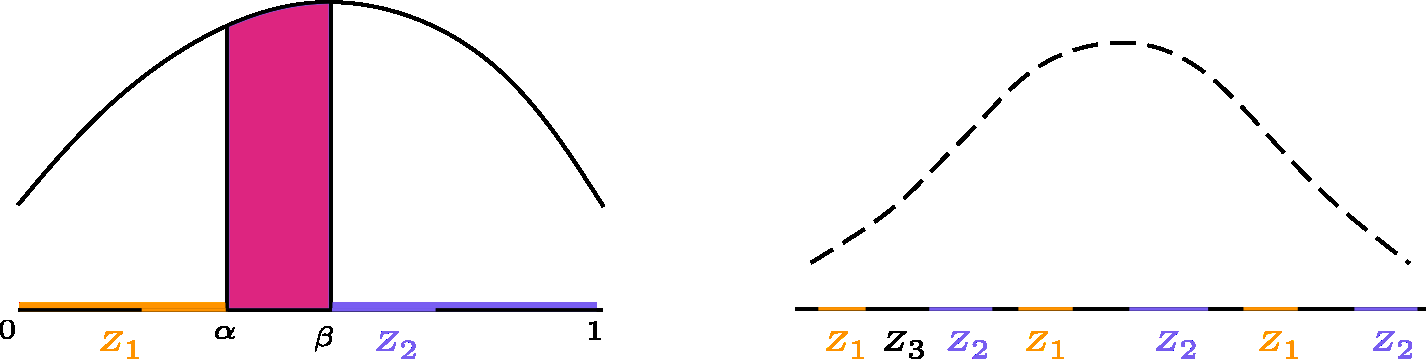
\includegraphics[width=0.5\textwidth]{Figures/concave-to-affine}\caption{Going to an affine needle}
\end{figure}

The overall proof idea is to subdivide $K'$ with a hyperplane in
such a way that one of the resulting halfspaces satisfies the same
two inequalities but violates either (i) or (ii). To choose this hyperplane,
we first fix an $(n-2)$-dimensional subspace $A=\left\{ x:x_{1}=\sigma,\,x_{2}+\ldots+x_{n}=\tau\right\} $
where $0<\sigma<1$ and $\tau>0$. The hyperplane will be chosen to
contain $A$ and bisect the function $\hat{g}$ so that $\int_{L}\hat{g}=\int_{L'}\hat{g}=0$
in both resulting convex bodies $L$ and $L'$. Suppose $\int_{L}h\ge0$.
Then we can infer that $L$ must intersect both $Z_{0}$ and $Z_{1}$,
otherwise the function $\psi$ restricted to $L$ contradicts the
(i), the minimality of the support of $\psi$. 

We now consider 3 cases:
\begin{enumerate}
\item $\psi(0)=\psi(1)=0$. For this case, let $\sigma=1/2$. Then $L$
must contain the segment $[0,1]\,e_{1}$, for any $\tau>0$, else
it contradicts (i). Then there is a linear function $\ell(t)$ with
$\ell(0),\ell(1)\ge0,\ell(1/2)=\tau$ such that the function $\psi$
restricted to $L$ is $\psi_{L}(t)=\min\{\psi(t),\ell(t)\}$. But
then as $\tau\rightarrow0$, $\ell(t)$ tends to zero in the interval
$[0,1]$ and so $\psi_{L}$ is linear in a larger sub-interval tending
to $[0,1]$ contradicting (ii).
\item $\psi(0)=0,\psi(1)>0$. For this case, consider $\tau=\psi(1)\,\sigma$.
Now if $L$ does not contain $[0,1]\,e_{1}$, then $\psi_{L}(0)=\psi_{L}(1)=0$,
taking us back to the first case. Otherwise, $\psi_{L}$ is linear
in the interval $[\sigma,1]$ and hence for small enough $\sigma$
this again contradicts (ii).
\item $\psi(0),\psi(1)>0$. Consider the family of continuous, nonnegative,
convex functions $\eta:[0,1]\to\R_{+}$ satisfying $\eta(t)\le\psi(t)$
for all $t\in[0,1]$. Let 
\[
K_{\eta}=K'\cap\{x:x_{2}+\ldots+x_{n}\ge\eta(x_{1})\}=\{x\in\R_{+}:x_{1}\in[0,1],\,\eta(x_{1})\le x_{2}+\ldots+x_{n}\le\psi(x_{1})\}\,.
\]
Then we choose $\eta$ so that (iii) $\int^{1}_{0}\eta(t)\,dt$ is
maximal while still satisfying 
\[
\int_{\K_{\eta}}\hat{g}=0\,,\quad\int_{\K_{\eta}}\hat{h}\ge0\,.
\]
Then, we can assume that $\eta(0)<\psi(0),\eta(1)<\psi(1)$. If not,
we consider the function $\psi-\eta$ and this takes us back to one
of the previous cases. Now let $(\sigma,\tau)$ be the intersection
of the segments $[(0,\eta(0)),(1,\psi(1))]$ and $[(0,\psi(0)),(1,\eta(1))]$.
Let $M,M'$ be the partition of $K_{\eta}$ such that $M$ does not
contain $[0,1]\,e_{1}$ and
\[
\int_{M}\hat{g}=\int_{M'}\hat{g}=0\,.
\]
Then, if $\int_{M}\hat{h}\ge0$, this contradicts (iii), the maximality
of $\eta$. Hence, $\int_{M}\hat{h}<0$ and the truncated cone $K'\setminus M$
satisfies 
\[
\int_{K'\setminus M}\hat{g}=\int_{K'}\hat{g}-\int_{M}\hat{g}=0\qquad\int_{K'\setminus M}\hat{h}=\int_{K'}\hat{h}-\int_{M}\hat{h}\ge0\,,
\]
which contradicts (ii), the maximality of the linear subinterval of
$\psi$. 
\end{enumerate}
This completes the proof. 
\end{proof}
Going back to the proof of Theorem \ref{ISO2}, we can apply the localization
lemma to get an interval $[a,b]$ and an affine function $\ell$ such
that 
\begin{equation}
\int^{1}_{0}\ell(t)^{n-1}g((1-t)a+tb)\,dt>0\quad\mbox{ and }\quad\int^{1}_{0}\ell(t)^{n-1}h((1-t)a+tb)\,dt>0.\label{AFTERLEMMA}
\end{equation}
The functions $g,h$ as we have defined them are not lower semi-continuous.
However, this can be addressed by expanding $S_{1}$ and $S_{2}$
slightly so as to make them open sets, and making the support of $f$
an open set. Since we are proving strict inequalities, these modifications
do not affect the conclusion.

\begin{figure}[H]

\begin{centering}
\includegraphics[width=0.75\columnwidth]{Figures/Lemma_10\lyxdot 30}
\par\end{centering}
\centering{}
\end{figure}

Let us partition $[0,1]$ into $Z_{1},Z_{2},Z_{3}$ as follows: 
\[
Z_{i}=\{t\in[0,1]\,:\,(1-t)a+tb\in S_{i}\}.
\]
Note that for any pair of points $u\in Z_{1},v\in Z_{2},\,|u-v|\ge d(S_{1},S_{2})/D$.
We can rewrite (\ref{AFTERLEMMA}) as 
\[
\int_{Z_{3}}\ell(t)^{n-1}f((1-t)a+tb)\,dt<C\int_{Z_{1}}\ell(t)^{n-1}f((1-t)a+tb)\,dt
\]
and 
\[
\int_{Z_{3}}\ell(t)^{n-1}f((1-t)a+tb)\,dt<C\int_{Z_{2}}\ell(t)^{n-1}f((1-t)a+tb)\,dt.
\]
The functions $f$ and $\ell(\cdot)^{n-1}$ are both logconcave, so
$F(t)=\ell(t)^{n-1}f((1-t)a+tb)$ is also logconcave. We get, 
\begin{equation}
\int_{Z_{3}}F(t)\,dt<C\min\left\{ \int_{Z_{1}}F(t)\,dt,\int_{Z_{2}}F(t)\,dt\right\} .\label{FEQ}
\end{equation}
Now consider what Theorem \ref{ISO2} asserts for the function $F(t)$
over the interval $[0,1]$ and the partition $Z_{1},Z_{2},Z_{3}$:
\begin{equation}
\int_{Z_{3}}F(t)\,dt\geq2d(Z_{1},Z_{2})\min\left\{ \int_{Z_{1}}F(t)\,dt,\int_{Z_{2}}F(t)\,dt\right\} .\label{FEQ2}
\end{equation}
We have substituted $1$ for the diameter of the interval $[0,1]$.
Also, $2d(Z_{1},Z_{2})\geq2d(S_{1},S_{2})/D=C$. Thus, Theorem \ref{ISO2}
applied to the function $F(t)$ contradicts (\ref{FEQ}). To prove
the theorem in general, it suffices to prove it in the one-dimensional
case. A combinatorial argument reduces this to the case when each
$Z_{i}$ is a single interval. Proving the resulting inequality up
to a factor of $2$ is a simple exercise and uses only the unimodality
of $F$. The improvement to the tight bound requires one-dimensional
logconcavity. This completes the proof of Theorem \ref{ISO2}.

The localization lemma has been used to prove a variety of isoperimetric
inequalities. The next theorem is a refinement of Theorem \ref{ISO2},
replacing the diameter by the square-root of the expected squared
distance of a random point from the mean. For an isotropic distribution
this is an improvement from $n$ to $\sqrt{n}$. This theorem was
proved by Kannan-Lov�sz-Simonovits in the same paper in which they
proposed the KLS conjecture. 
\begin{thm}[\cite{Kannan1995}]
\label{thm:KLS_thm} For any logconcave density $p$ in $\R^{n}$
with covariance matrix $A$, the KLS constant satisfies
\[
\psi_{p}\gtrsim\frac{1}{\sqrt{\tr(A)}}.
\]
\end{thm}

The next theorem shows that the KLS conjecture is true for an important
family of distributions. The proof is again by localization \cite{CV2014},
and the one-dimensional inequality obtained is a Brascamp-Lieb Theorem.
We note that the same theorem can be obtained by other means \cite{Ledoux1999}.
\begin{thm}
\label{thm:Gaussian-iso}Let $h(x)=f(x)e^{-\frac{1}{2}x^{\top}Bx}/\int f(y)e^{-\frac{1}{2}y^{\top}By}dy$
where $f:\R^{n}\rightarrow\R_{+}$ is an integrable logconcave function
and $B$ is positive definite. Then $h$ is logconcave and for any
measurable subset $S$ of $\R^{n}$,
\[
\frac{h(\partial S)}{\min\left\{ h(S),h\left(\R^{n}\setminus S\right)\right\} }\gtrsim\frac{1}{\norm{B^{-1}}^{\frac{1}{2}}_{\op}}.
\]
In other words, the expansion of h is $\Omega(\norm{B^{-1}}^{-\frac{1}{2}}_{\op})$.
\end{thm}

The analysis of the Gaussian Cooling algorithm for volume computation
\cite{CV2015} uses localization.

Next we mention an application to the anti-concentration of polynomials.
This is a corollary of a more general result by Carbery and Wright.
\begin{thm}[\cite{carbery2001distributional}]
Let $q$ be a degree $d$ polynomial in $\R^{n}$. Then for a convex
body $K\subset\R^{n}$ of volume $1$, any $\epsilon>0$, and $x$
drawn uniformly from $K$, 
\[
\Pr_{x\sim K}\left(|q(x)|\le\epsilon\max_{K}|q(x)|\right)\lesssim\epsilon^{\frac{1}{d}}d
\]
\end{thm}


\subsection{Alternative formulations of Localization}

Here we give some alternative equivalent versions of Lemma \ref{lem:LOCALIZATION}
which are sometimes more convenient in applications.

The first is in terms of single inequality on products of integrals.
Note that an $n$-dimensional needle $N$ is specified by a pair of
points $a,b\in\R^{n}$ and a linear function $\ell:[0,1]\rightarrow\R_{+}$.
The integral over a needle is defined as 
\[
\int_{N}f=\int^{1}_{0}f((1-t)a+tb)\ell(t)^{n-1}\,dt.
\]

\begin{lem}[Localization: Product form]
 Let $f_{1},f_{2},f_{3},f_{4}:\R^{n}\rightarrow\R_{+}$ be nonnegative,
continuous functions. Then the following are equivalent:
\end{lem}

\begin{enumerate}
\item For every convex body $K\subset\R^{n},$ we have
\[
\int_{K}f_{1}\int_{K}f_{2}\le\int_{K}f_{3}\int_{K}f_{4}.
\]
\item For every needle $N$ in $\R^{n}$, we have
\[
\int_{N}f_{1}\int_{N}f_{2}\le\int_{N}f_{3}\int_{N}f_{4}.
\]
\end{enumerate}
The next version is in terms of exponential needles, i.e., we replace
the linear functions obtained in the one-dimensional case in Lemma
\ref{lem:LOCALIZATION} with truncated exponentials. 
\begin{lem}[Localization: exponential needles]
\label{lem:localization_exp_needles} Let $f_{1},f_{2},f_{3},f_{4}:\R^{n}\rightarrow\R_{+}$
be nonnegative, continuous functions and $\alpha,\beta>0$. Then,
the following are equivalent:
\end{lem}

\begin{enumerate}
\item For every logconcave function $F:\R^{n}\rightarrow\R_{+}$, we have
\[
\left(\int_{\R^{n}}F(x)\,f_{1}(x)\,dx\right)^{\alpha}\left(\int_{\R^{n}}F(x)\,f_{2}(x)\,dx\right)^{\beta}\le\left(\int_{\R^{n}}F(x)\,f_{3}(x)\,dx\right)^{\alpha}\left(\int_{\R^{n}}F(x)\,f_{4}(x)\,dx\right)^{\beta}\,.
\]
\item For every interval $a,b\in\R^{n}$ and every $\gamma\in\R$, we have
\[
\left(\int^{1}_{0}e^{\gamma t}f_{1}(t)\,dt\right)^{\alpha}\left(\int^{1}_{0}e^{\gamma t}f_{2}(t)\,dt\right)^{\beta}\le\left(\int^{1}_{0}e^{\gamma t}f_{3}(t)\,dt\right)^{\alpha}\left(\int^{1}_{0}e^{\gamma t}f_{4}(t)\,dt\right)^{\beta}\,
\]
where $f_{i}(t)=f_{i}((1-t)a+tb)$.
\end{enumerate}
\begin{rem}
We can also write the exponential needle version of localization in
terms of two inequalities or one equality and one inequality: For
every logconcave $\ensuremath{F:\R\rightarrow\R_{+}}$
\[
\int^{b}_{a}Ff_{1}=0,\ \int^{b}_{a}Ff_{2}>0
\]
if and only if for every subinterval $\ensuremath{[a',b']\subseteq[a,b]}$,
and every $\gamma\in\R$, 
\[
\int^{b'}_{a'}e^{\gamma t}f_{1}=0,\ \int^{b'}_{a'}e^{\gamma t}f_{2}>0.
\]

We conclude this section with a nice interpretation of the localization
lemma by Fradelizi and Guedon. They also give a version that extends
localization to multiple inequalities.
\end{rem}

\begin{thm}[Reformulated Localization Lemma \cite{fradelizi2004extreme}]
Let $K$ be a compact convex set in $\Rn$ and $f$ be an upper semi-continuous
function. Let $P_{f}$ be the set of logconcave distributions $\mu$
supported by $K$ satisfying $\int fd\mu\geq0$. The set of extreme
points of $\text{conv}\,P_{f}$ is exactly:
\begin{enumerate}
\item the Dirac measure at points $x$ such that $f(x)\geq0$, or
\item the distributions $v$ that satisfy
\begin{enumerate}
\item density function is of the form $e^{\ell}$ with linear $\ell$,
\item support is a segment $[a,b]\subset K$,
\item $\int fdv=0$,
\item $\int^{x}_{a}fdv>0$ for $x\in(a,b)$ or $\int^{b}_{x}fdv>0$ for
$x\in(a,b)$.
\end{enumerate}
\end{enumerate}
\end{thm}

Since we know the maximizer of any convex function is at extreme points,
this shows that one can optimize $\max_{\mu\in P_{f}}\Phi(\mu)$ for
any convex $\Phi$ by only checking Dirac measures and log-affine
functions.
